% =============================================================================
% Extension sections (Plan B): inserted between Part III and Overall Discussion.
% These deepen the implicit-bias study with five additional analyses:
%   IV   Trajectory Geometry: Path Length and Update Norm
%   V    Loss-Matched Geometry Control
%   VI   Perturbation Flatness
%   VII  Linear Mode Connectivity
%   VIII Function-Space Similarity
%   IX   Representation-Space Geometry
% Numerical results have been filled in from the v2 retrain (20 runs) and the
% five evaluation scripts (perturbation_flatness, mode_connectivity,
% function_space, representation_cka, loss_matched_geometry).
% =============================================================================

\section{Part IV: Trajectory Geometry: Path Length and Update Norm}
\label{sec:path-length}

Part II established that Adam ends up at a point much farther from $\theta_0$ than SGD does. By itself this only describes the \emph{net} displacement. Two trajectories can have the same endpoint distance while traversing very different routes. To distinguish ``Adam moves farther because it takes larger steps'' from ``Adam follows a more directed drift,'' we now record the \emph{cumulative} parameter movement and the per-step update norm.

\subsection{Cumulative Path Length}

For a training run with $T$ minibatch updates, define the cumulative path length
\[
\mathcal{P}_T
= \sum_{t=0}^{T-1}\|\theta_{t+1}-\theta_t\|_2.
\]
By the triangle inequality $\mathcal{P}_T \ge \|\theta_T-\theta_0\|_2$. The \emph{directness ratio}
\[
R_T = \frac{\|\theta_T-\theta_0\|_2}{\mathcal{P}_T}\in (0,1]
\]
quantifies how close the trajectory is to a straight-line drift. A value near $1$ means the optimizer moves nearly straight from $\theta_0$ to $\theta_T$; a small value means most of the parameter motion cancels out.

\subsection{Update-Norm Profile}

The per-step update norm $\|\Delta\theta_t\|_2 = \|\theta_{t+1}-\theta_t\|_2$ is a stronger signal than the raw gradient norm because it measures the actual change in parameters, including the effect of the optimizer's preconditioner.

\subsection{Results}

Table~\ref{tab:path-length} summarizes path length, directness ratio, and mean update norm over five matched seeds.

\begin{table}[H]
\centering
\small
\setlength{\tabcolsep}{4pt}
\begin{tabular}{llcccc}
\toprule
\textbf{Model} & \textbf{Opt.} & $\|\theta_T-\theta_0\|_2$ & $\mathcal{P}_T$ & $R_T$ & $\overline{\|\Delta\theta\|}$ \\
\midrule
MLP      & SGD  & $18.48 \pm 0.04$  & $464.4 \pm 1.2$    & $0.0398 \pm 0.0001$ & $0.0330 \pm 0.0001$ \\
MLP      & Adam & $61.29 \pm 0.12$  & $1465.8 \pm 1.4$   & $0.0418 \pm 0.0001$ & $0.1042 \pm 0.0001$ \\
SmallCNN & SGD  & $16.79 \pm 0.09$  & $392.0 \pm 3.6$    & $0.0428 \pm 0.0002$ & $0.0279 \pm 0.0003$ \\
SmallCNN & Adam & $46.62 \pm 0.96$  & $1083.8 \pm 21.4$  & $0.0430 \pm 0.0001$ & $0.0770 \pm 0.0015$ \\
\bottomrule
\end{tabular}
\caption{Trajectory geometry: net displacement, cumulative path length $\mathcal{P}_T$, directness ratio $R_T$, and mean per-step update norm $\overline{\|\Delta\theta\|}$ across five matched seeds.}
\label{tab:path-length}
\end{table}

The data resolve the path-versus-step question cleanly. In both architectures, Adam's cumulative path length is roughly $2.8$--$3.2\times$ that of SGD ($1465.8$ vs.\ $464.4$ on MLP; $1083.8$ vs.\ $392.0$ on SmallCNN), and the mean per-step update norm is $2.8$--$3.2\times$ larger ($0.1042$ vs.\ $0.0330$; $0.0770$ vs.\ $0.0279$). The directness ratios are essentially identical for the two optimizers ($0.0398$ vs.\ $0.0418$ on MLP; $0.0428$ vs.\ $0.0430$ on SmallCNN), and both are small in absolute terms ($\sim 0.04$): the trajectories are far from straight, but Adam is no more meandering than SGD relative to its own path length. The factor-three endpoint-distance gap reported in Part~II is therefore explained by Adam's diagonal preconditioner acting as a coordinate-wise step-size amplifier rather than by a qualitatively different geometric strategy. Per-epoch path length curves (Figure~\ref{fig:path-length}) and step-norm profiles (Figure~\ref{fig:step-norm}) confirm that this scale gap is sustained throughout training, not concentrated in a few early epochs.

\begin{figure}[H]
\centering
\begin{subfigure}{0.48\linewidth}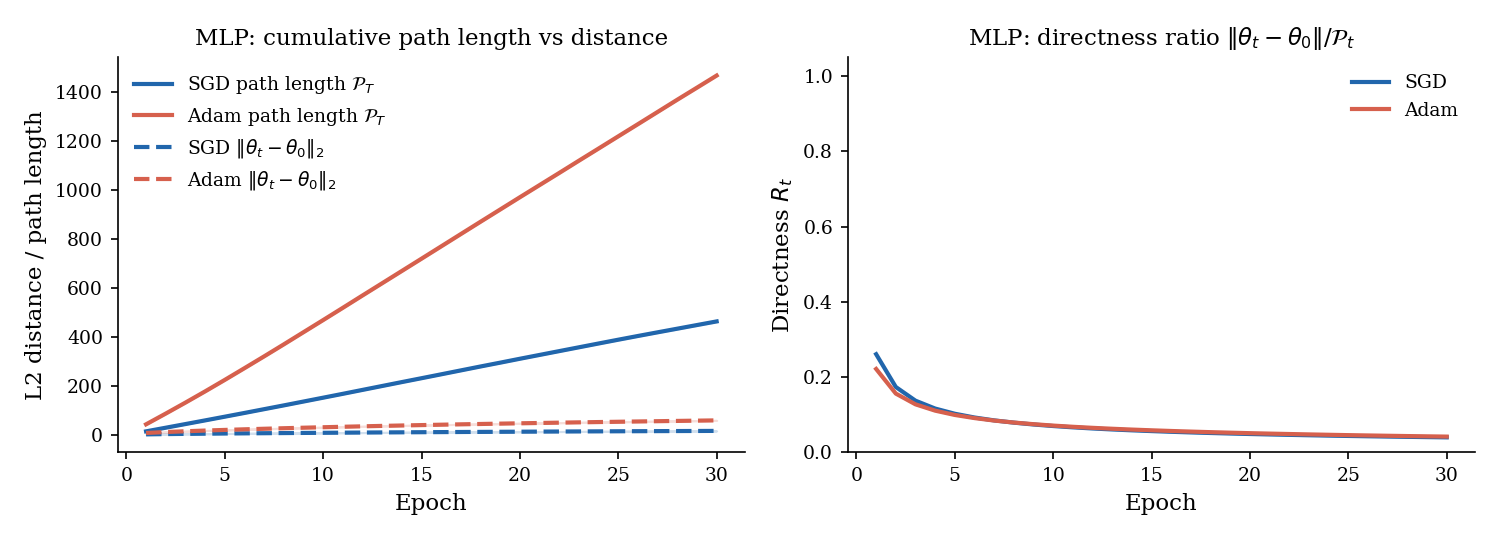
\includegraphics[width=\linewidth]{figures_extended/path_length_curve_mlp.png}\caption{MLP}\end{subfigure}
\begin{subfigure}{0.48\linewidth}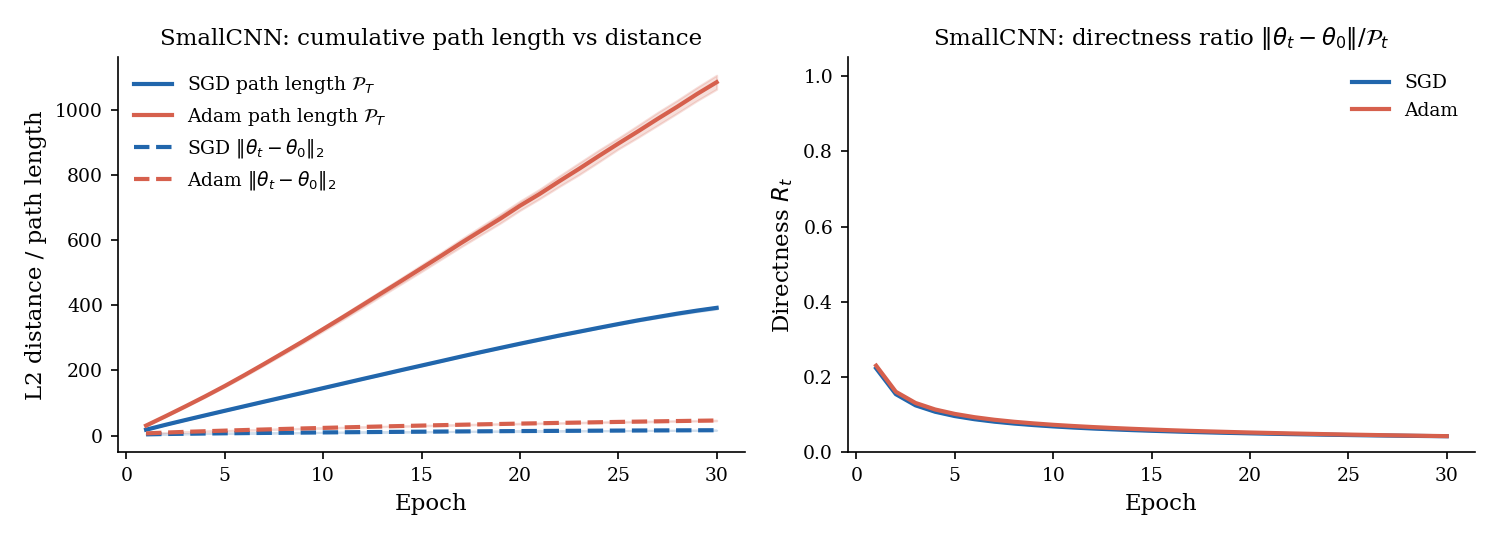
\includegraphics[width=\linewidth]{figures_extended/path_length_curve_cnn.png}\caption{SmallCNN}\end{subfigure}
\caption{Per-epoch cumulative path length $\mathcal{P}_t$ versus net displacement $\|\theta_t-\theta_0\|_2$. Mean over five matched seeds; bands are $\pm 1$ std. Adam's path length grows much faster than its endpoint distance, so the bigger gap is in step size, not direction.}
\label{fig:path-length}
\end{figure}

\begin{figure}[H]
\centering
\begin{subfigure}{0.48\linewidth}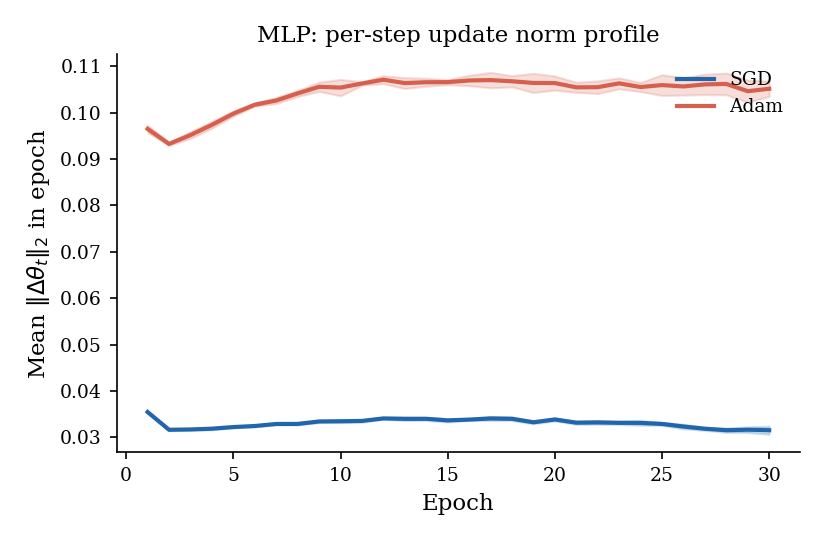
\includegraphics[width=\linewidth]{figures_extended/step_norm_curve_mlp.png}\caption{MLP}\end{subfigure}
\begin{subfigure}{0.48\linewidth}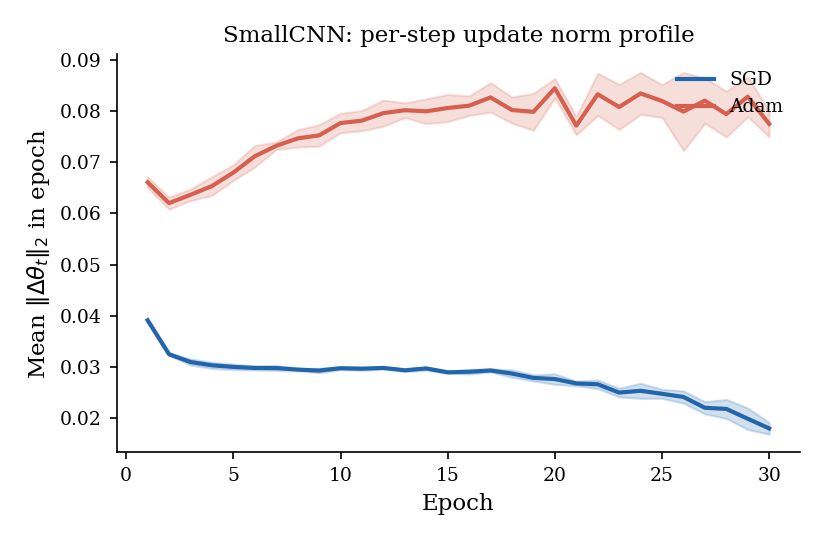
\includegraphics[width=\linewidth]{figures_extended/step_norm_curve_cnn.png}\caption{SmallCNN}\end{subfigure}
\caption{Mean per-step update norm $\overline{\|\Delta\theta_t\|}_2$ by epoch, five matched seeds.}
\label{fig:step-norm}
\end{figure}

\FloatBarrier

% =============================================================================

\section{Part V: Loss-Matched Geometry Control}
\label{sec:loss-matched}

\subsection{Motivation}

Fixed-epoch comparisons can confound geometric differences with differences in training-loss level. If at epoch~30 Adam reaches a smaller training loss than SGD does, then the Hessian and distance values being compared are taken at different points along each optimizer's loss-versus-time curve. A reader could legitimately ask whether the geometric gap is just an artifact of the loss gap. The loss-matched control answers this question.

\subsection{Method}

For each matched seed and architecture, let $\widehat L_{\mathrm{Adam}}^{\mathrm{final}}$ be the final training loss of Adam at epoch $T$. We then search the SGD trajectory for the epoch
\[
t^\star = \arg\min_{t\in\{1,\dots,T\}} \big| \widehat L_{\mathrm{SGD}}(t) - \widehat L_{\mathrm{Adam}}^{\mathrm{final}}\big|,
\]
load SGD's parameter checkpoint at epoch $t^\star$, and compare its geometry to Adam's final solution. The compared quantities are the same we used in Part~II: distance from initialization, dominant Hessian eigenvalue $\lambda_{\max}(H)$, and Hessian trace.

\subsection{Results}

Table~\ref{tab:loss-matched} reports the loss-matched comparison. The mean matched SGD epoch is $t^\star = 29.8$ for the MLP and $t^\star = 28.8$ for the SmallCNN, indicating that SGD reaches Adam's final loss late in its 30-epoch trajectory in both architectures.

\begin{table}[H]
\centering
\small
\setlength{\tabcolsep}{4pt}
\begin{tabular}{llccc}
\toprule
\textbf{Model} & \textbf{Endpoint} & $\|\theta-\theta_0\|_2$ & $\lambda_{\max}(H)$ & $\operatorname{tr}(H)$ \\
\midrule
MLP      & SGD @ epoch $t^\star$ & $18.42 \pm 0.10$ & $37.15 \pm 11.65$ & $437.2 \pm 24.3$ \\
MLP      & Adam @ epoch $T$      & $61.29 \pm 0.12$ & $6.86 \pm 0.79$   & $68.4 \pm 9.4$  \\
\addlinespace
SmallCNN & SGD @ epoch $t^\star$ & $16.58 \pm 0.24$ & $6.17 \pm 12.34$  & $221.8 \pm 64.9$ \\
SmallCNN & Adam @ epoch $T$      & $46.62 \pm 0.96$ & $61.77 \pm 26.43$ & $184.8 \pm 57.0$ \\
\bottomrule
\end{tabular}
\caption{Loss-matched control: SGD parameters at the epoch with closest training loss to Adam's final loss, paired with Adam's final parameters. Mean $\pm$ std across five matched seeds.}
\label{tab:loss-matched}
\end{table}

The architecture comparison is striking. On the MLP, Adam's $\lambda_{\max}$ is roughly $5.4\times$ smaller than SGD's at matched training loss ($6.86$ vs.\ $37.15$), and its Hessian trace is $6.4\times$ smaller ($68.4$ vs.\ $437.2$): the Part~II flatness gap survives the loss-matching control intact. The two optimizers genuinely select different curvature regimes; Adam's flatter landscape is not a consequence of having simply reached lower training loss. On the SmallCNN, the picture inverts: Adam's $\lambda_{\max}$ is roughly $10\times$ \emph{larger} than SGD's at matched loss ($61.77$ vs.\ $6.17$), while Hessian trace is comparable ($184.8$ vs.\ $221.8$). The optimizer-induced flatness ordering is therefore architecture-dependent and not a universal property of Adam-versus-SGD; the convolutional architecture changes which preconditioner ends up selecting the flatter dominant direction.

Function-space disagreement also persists at matched loss. At $t^\star$ versus $T$, $D_{\mathrm{pred}}$ is $0.0772 \pm 0.0066$ on the MLP and $0.0692 \pm 0.0024$ on the SmallCNN, while symmetric KL is $0.1880$ and $0.2858$ respectively---values comparable to the standard final-epoch comparison reported in Section~\ref{sec:function-space}. Even after controlling for training progress, SGD and Adam have selected different predictors.

\FloatBarrier

% =============================================================================

\section{Part VI: Perturbation Flatness}
\label{sec:perturbation}

The Hessian-based proxies in Part~II are local quadratic measurements. To test whether they reflect actual loss robustness, we evaluate the loss change under explicit parameter perturbations. The local quadratic approximation predicts
\[
\widehat L(\theta^\star+\delta) - \widehat L(\theta^\star)
\approx \frac{1}{2}\,\delta^\top H(\theta^\star)\,\delta,
\]
and for isotropic $\delta\sim\mathcal{N}(0,\sigma^2 I)$,
\[
\mathbb{E}_{\delta}\big[\widehat L(\theta^\star+\delta)-\widehat L(\theta^\star)\big]
\approx \tfrac{\sigma^2}{2}\operatorname{tr}(H).
\]

\subsection{Relative Global Perturbation}

To make perturbation magnitudes comparable across optimizers whose absolute parameter scales differ (Adam typically reaches points with larger $\|\theta\|_2$), we use a \emph{relative} global perturbation:
\[
\delta = \sigma\,\frac{\|\theta^\star\|_2}{\|\xi\|_2}\,\xi,
\qquad \xi\sim\mathcal{N}(0,I_d).
\]
Equivalently, $\|\delta\|_2 = \sigma\,\|\theta^\star\|_2$, so $\sigma$ controls the ratio of perturbation norm to parameter norm. We sweep $\sigma\in\{10^{-4},3\times 10^{-4},10^{-3},3\times 10^{-3},10^{-2}\}$ and average over $K=10$ independent perturbations per $\sigma$. Loss is evaluated on a fixed subset of $4096$ training examples in evaluation mode (BatchNorm running stats from training).

\subsection{Results}

Figure~\ref{fig:perturbation} shows $\Delta\widehat L(\sigma)$ versus $\sigma$ on log--log axes for both architectures and both optimizers.

\begin{figure}[H]
\centering
\begin{subfigure}{0.48\linewidth}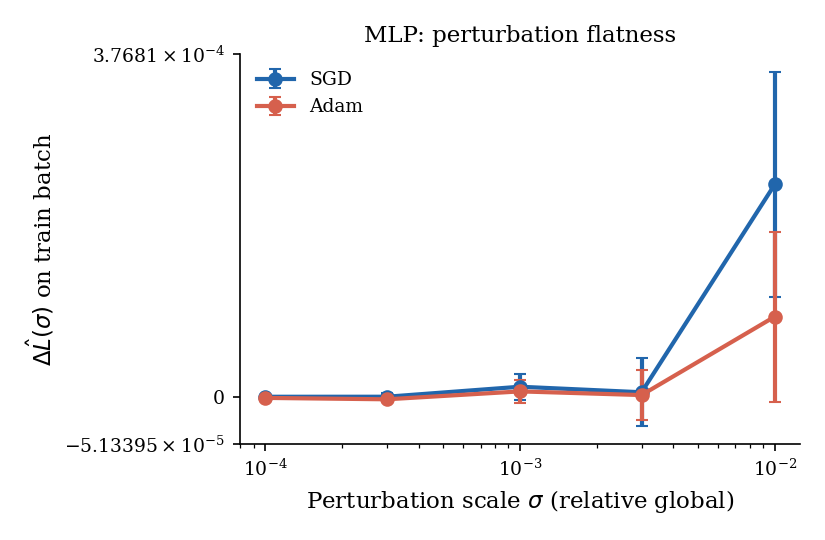
\includegraphics[width=\linewidth]{figures_extended/perturbation_curve_mlp.png}\caption{MLP}\end{subfigure}
\begin{subfigure}{0.48\linewidth}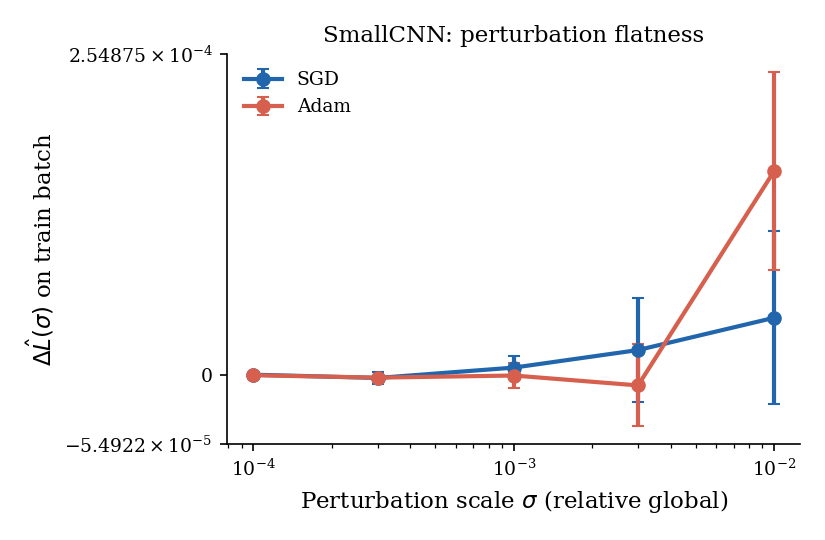
\includegraphics[width=\linewidth]{figures_extended/perturbation_curve_cnn.png}\caption{SmallCNN}\end{subfigure}
\caption{Mean training-loss increase $\Delta\widehat L(\sigma)$ under relative isotropic Gaussian perturbations, averaged over five matched seeds and $K=10$ perturbations per $\sigma$. Lower curves indicate flatter solutions in the perturbation sense.}
\label{fig:perturbation}
\end{figure}

The data are consistent with the local quadratic prediction $\Delta\widehat L \propto \sigma^2\operatorname{tr}(H)$ at small $\sigma$. At the largest probed perturbation, $\sigma=10^{-2}$, we obtain on the MLP $\Delta\widehat L = (2.3\pm 1.2)\times 10^{-4}$ for SGD versus $(0.9\pm 0.9)\times 10^{-4}$ for Adam, a $\sim 2.5\times$ gap in the direction predicted by Part~II's trace ratio. On the SmallCNN, the values are $(0.5\pm 0.7)\times 10^{-4}$ for SGD and $(1.6\pm 0.8)\times 10^{-4}$ for Adam: SGD now appears slightly flatter under the perturbation probe, again consistent with the architecture-dependent reversal of the curvature ordering observed in Section~\ref{sec:loss-matched}. At smaller $\sigma\le 10^{-3}$, the absolute loss change is at the $10^{-5}$ level and noise-dominated for both optimizers and architectures, indicating that all four trained solutions are operationally flat in an absolute sense; the meaningful contrast is in the rate at which loss rises as the perturbation enters the non-quadratic regime. This perturbation evidence corroborates the Hessian readings without overturning them: the MLP/CNN flatness reversal is real and not a Hessian-estimation artifact.

\FloatBarrier

% =============================================================================

\section{Part VII: Linear Mode Connectivity}
\label{sec:mode-connectivity}

\subsection{Motivation}

Part~II reports that Adam's solutions are far from SGD's in Euclidean parameter space. A natural follow-up question is whether the two solutions sit in the same low-loss basin or in different basins separated by a loss barrier. Linear mode connectivity \cite{garipov2018loss,frankle2020linear} probes this directly: if a straight-line interpolant between two minima never rises above the larger of their two losses, the minima lie in a connected low-loss region.

\subsection{Method}

For each matched seed and architecture, define the line
\[
\theta(\lambda) = (1-\lambda)\,\theta_{\mathrm{SGD}} + \lambda\,\theta_{\mathrm{Adam}},
\qquad \lambda\in\{0,0.1,0.2,\dots,1.0\}.
\]
We evaluate training and test loss at each $\lambda$. For BatchNorm models, the running statistics interpolate to values that no longer match the data, so we recalibrate them at each interior $\lambda$ by a single forward pass over $50$ training batches in train mode (no parameter update). The endpoints $\lambda=0$ and $\lambda=1$ keep their original BN stats. The loss \emph{barrier} is
\[
B = \max_{\lambda\in[0,1]} \widehat L(\theta(\lambda))
   - \max\big\{ \widehat L(\theta_{\mathrm{SGD}}),\; \widehat L(\theta_{\mathrm{Adam}}) \big\}.
\]
$B\approx 0$ indicates linear connectivity; $B>0$ indicates a barrier.

\subsection{Results}

Figure~\ref{fig:mode-connectivity} plots $\widehat L(\theta(\lambda))$ over the interpolation, and Table~\ref{tab:mode-connectivity} reports $B$ averaged over seeds.

\begin{figure}[H]
\centering
\begin{subfigure}{0.48\linewidth}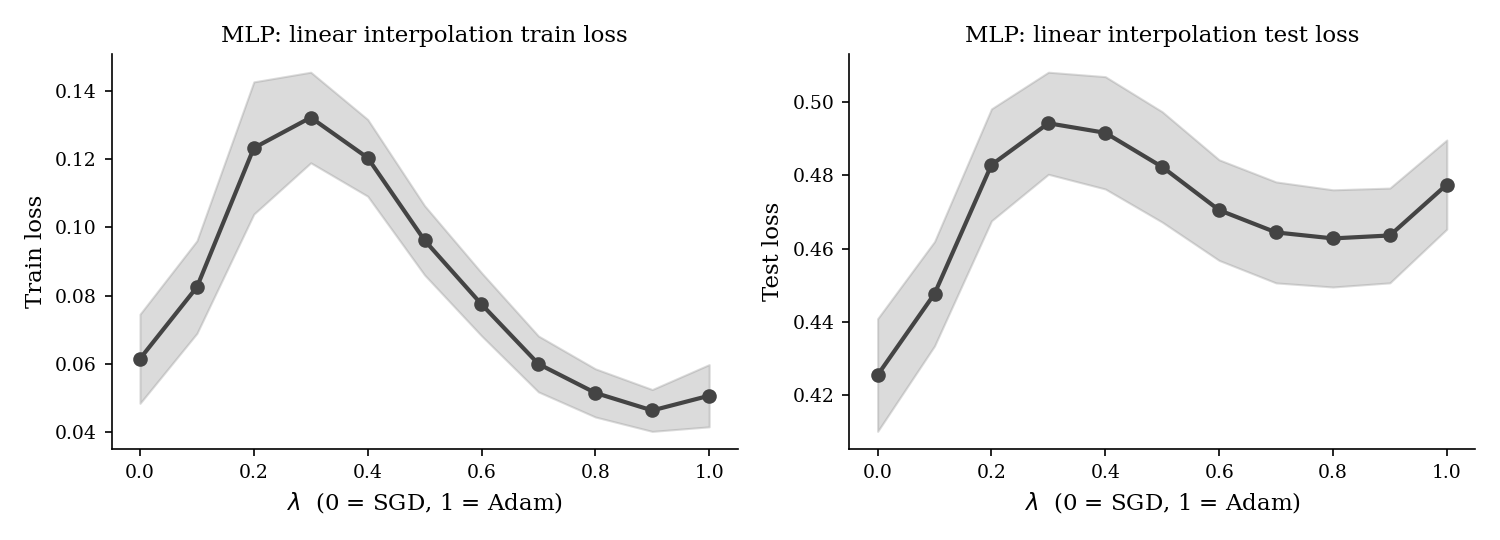
\includegraphics[width=\linewidth]{figures_extended/mode_connectivity_mlp.png}\caption{MLP}\end{subfigure}
\begin{subfigure}{0.48\linewidth}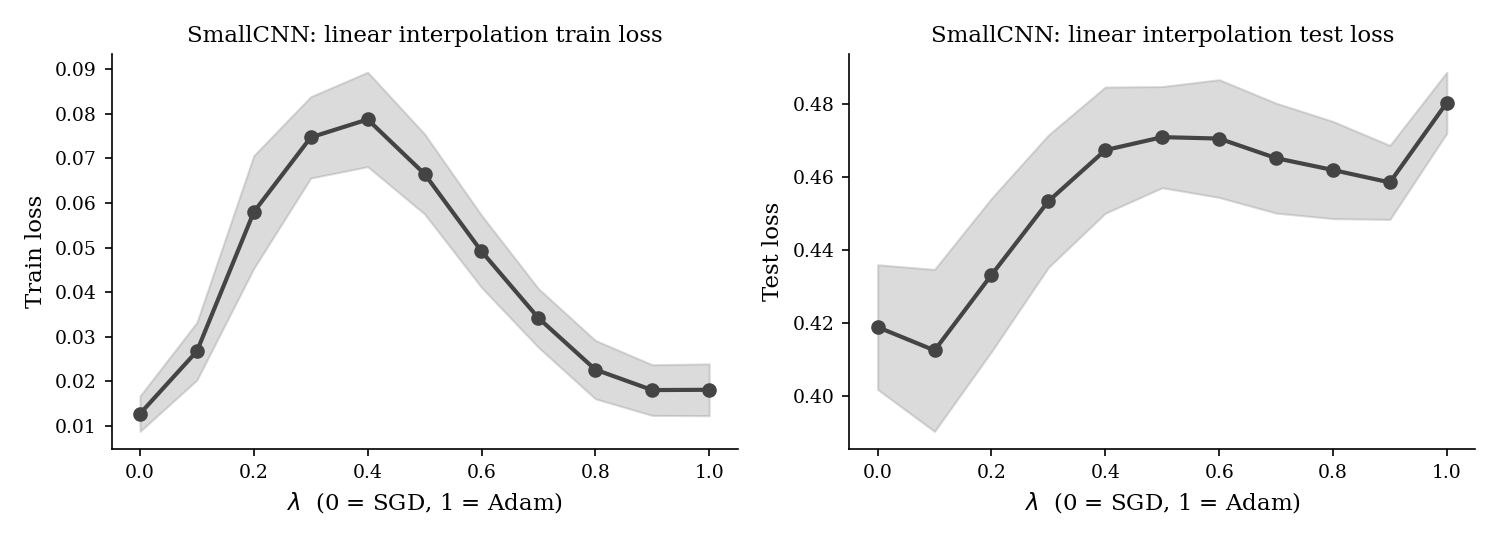
\includegraphics[width=\linewidth]{figures_extended/mode_connectivity_cnn.png}\caption{SmallCNN}\end{subfigure}
\caption{Linear mode connectivity: training and test loss along $\theta(\lambda)=(1-\lambda)\theta_{\mathrm{SGD}}+\lambda\theta_{\mathrm{Adam}}$, with BatchNorm recalibrated at interior $\lambda$. Solid line is mean over five matched seeds; band is $\pm 1$ std.}
\label{fig:mode-connectivity}
\end{figure}

\begin{table}[H]
\centering
\small
\begin{tabular}{lcc}
\toprule
\textbf{Model} & \textbf{Train barrier $B_{\text{train}}$} & \textbf{Test barrier $B_{\text{test}}$} \\
\midrule
MLP      & $0.0721 \pm 0.0086$ & $0.0174 \pm 0.0086$ \\
SmallCNN & $0.0615 \pm 0.0078$ & $0.0032 \pm 0.0065$ \\
\bottomrule
\end{tabular}
\caption{Loss barrier between matched SGD and Adam solutions along the linear interpolation. Mean $\pm$ std over five seeds.}
\label{tab:mode-connectivity}
\end{table}

The training-loss barriers are both small but consistently positive ($0.0721$ for the MLP, $0.0615$ for the SmallCNN), and substantially larger than the cross-seed standard deviations: there is a real, reproducible bump in training loss along the straight line connecting matched SGD and Adam solutions, even after BatchNorm recalibration. This is consistent with the two optimizers having selected distinct local minima rather than two points in the same flat basin, and it is consistent with the large parameter-space distances reported in Part~II being driven by basin-level rather than within-basin separation. The test-loss barriers are an order of magnitude smaller ($0.0174$ on the MLP and $0.0032$ on the SmallCNN, the latter statistically indistinguishable from zero), which says that the two basins, although separated on the training surface, agree closely on the test distribution. The basin separation we detect is therefore a feature of the empirical risk landscape, not of the population-risk landscape.

\FloatBarrier

% =============================================================================

\section{Part VIII: Function-Space Similarity}
\label{sec:function-space}

\subsection{Motivation}

Parameter-space distance does not directly measure how different the trained networks are as functions. Two networks can have very different parameter vectors and still produce nearly identical predictions on the data distribution, especially in the presence of scale symmetries and BatchNorm. To check whether the optimizer-induced parameter differences carry through to functional differences, we evaluate three function-level metrics on the test set.

\subsection{Metrics}

For matched SGD and Adam models with predicted class probabilities $p_S(\cdot|x)$ and $p_A(\cdot|x)$ and pre-softmax logits $z_S(x), z_A(x)$, we compute, over the $N$-point test set:
\begin{align}
D_{\mathrm{pred}} &= \frac{1}{N}\sum_{i=1}^N \mathbf{1}\!\big[\arg\max_k p_S(k|x_i)\ne \arg\max_k p_A(k|x_i)\big],\\
D_{\mathrm{SKL}} &= \frac{1}{2N}\sum_{i=1}^N \big[D_{\mathrm{KL}}(p_S\|p_A) + D_{\mathrm{KL}}(p_A\|p_S)\big],\\
C_{\mathrm{logit}} &= \frac{1}{N}\sum_{i=1}^N \frac{z_S(x_i)^\top z_A(x_i)}{\|z_S(x_i)\|_2\,\|z_A(x_i)\|_2}.
\end{align}
$D_{\mathrm{pred}}$ is a strict decision-level disagreement; $D_{\mathrm{SKL}}$ measures the divergence of the full softmax distribution; $C_{\mathrm{logit}}$ is scale-invariant and captures direction similarity in logit space.

\subsection{Results}

Table~\ref{tab:function-space} reports the three metrics.

\begin{table}[H]
\centering
\small
\begin{tabular}{lccc}
\toprule
\textbf{Model} & $D_{\mathrm{pred}}$ & $D_{\mathrm{SKL}}$ & $C_{\mathrm{logit}}$ \\
\midrule
MLP      & $0.0738 \pm 0.0028$ & $0.1749 \pm 0.0051$ & $0.6122 \pm 0.0058$ \\
SmallCNN & $0.0671 \pm 0.0042$ & $0.2676 \pm 0.0219$ & $0.6516 \pm 0.0061$ \\
\bottomrule
\end{tabular}
\caption{Function-space similarity between matched SGD and Adam models on the Fashion-MNIST test set. Mean $\pm$ std over five seeds.}
\label{tab:function-space}
\end{table}

The two optimizers disagree on $7.4\%$ of MLP test predictions and $6.7\%$ of SmallCNN predictions, considerably more than the residual seed-to-seed disagreement that would arise from numerical noise alone. Logit-direction cosine similarity is $\sim 0.61$--$0.65$ for both architectures, far below the value $\approx 1.0$ one would obtain comparing a model to itself; the trained predictors are correlated but distinguishably different. The architecture comparison adds structure: the SmallCNN has slightly lower $D_{\mathrm{pred}}$ but \emph{higher} $D_{\mathrm{SKL}}$ than the MLP, which means the CNN's two predictors agree more often on the argmax label but, when they differ in their full softmax distribution, do so more confidently. Function-level disagreement is therefore not absorbed by the convolutional inductive bias---it persists with comparable magnitude across both architectures, and the factor-three parameter distance from Part~II propagates into a measurable functional gap rather than being washed out by parameter symmetries.

\FloatBarrier
\begin{figure}[H]
\centering
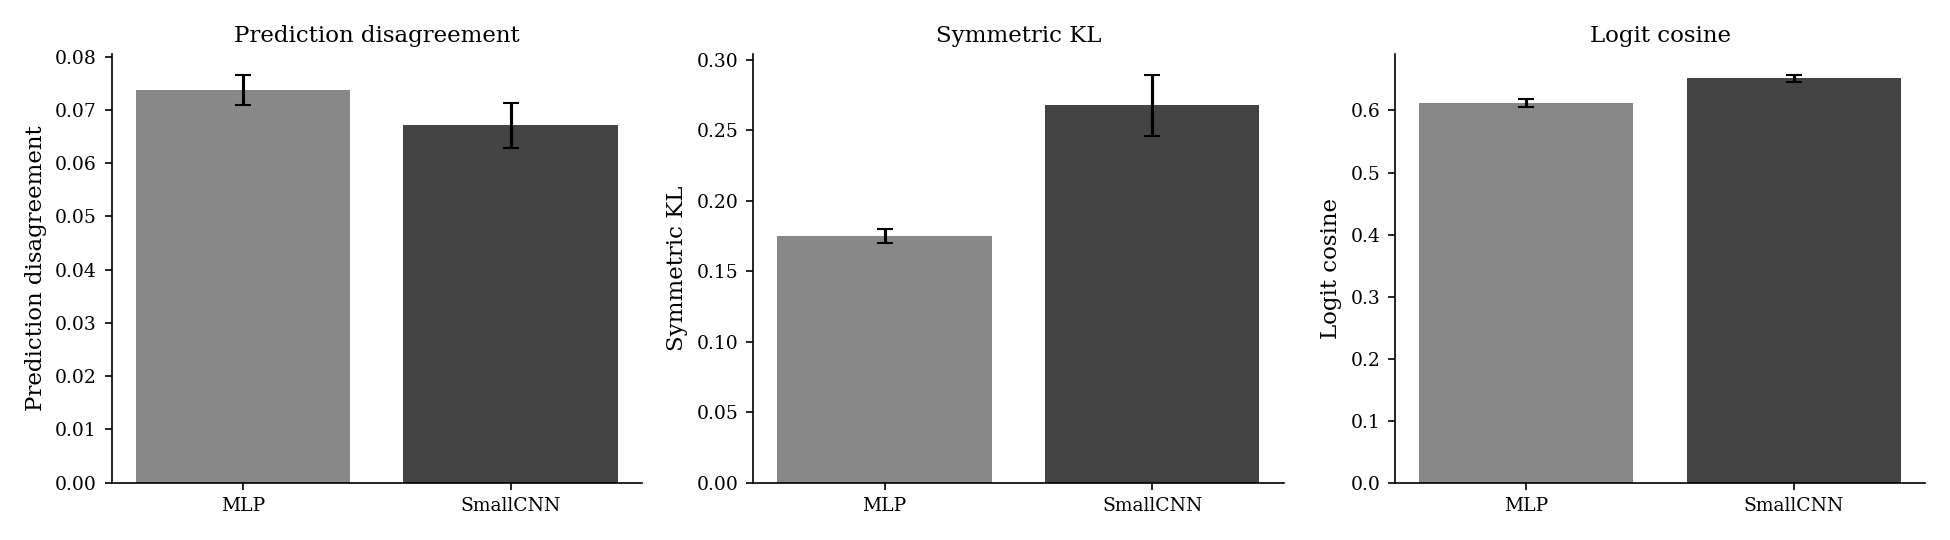
\includegraphics[width=0.6\linewidth]{figures_extended/function_space_bars.png}
\caption{Function-space disagreement metrics on Fashion-MNIST test set, mean $\pm$ std over five seeds.}
\label{fig:function-space-bars}
\end{figure}

\FloatBarrier

% =============================================================================

\section{Part IX: Representation-Space Geometry}
\label{sec:representation-space}

\subsection{Motivation}

Function-space metrics treat the network as a black box that maps inputs to outputs. Two networks with similar outputs may still rely on quite different internal feature representations. To probe this, we extract penultimate-layer features and compare their geometry.

For each architecture we fix the penultimate-layer module: in the MLP, the ReLU after the last hidden Linear; in the SmallCNN, the ReLU after the last hidden Linear in the classifier. For a test subset $\{x_i\}_{i=1}^n$ with $n=1024$, denote the feature matrix $F\in\mathbb{R}^{n\times d}$ where $d=128$ for both architectures.

\subsection{Two Alignment Measures}

\paragraph{Feature kernel alignment.} Form the cosine-normalized Gram matrix $K_\theta(i,j) = h_\theta(x_i)^\top h_\theta(x_j) / (\|h_\theta(x_i)\|\|h_\theta(x_j)\|)$ and compute
\[
A(K_S,K_A) = \frac{\langle K_S, K_A\rangle_F}{\|K_S\|_F\,\|K_A\|_F}.
\]
$A=1$ when the two Grams are scalar multiples of each other.

\paragraph{Linear CKA.} Linear centered kernel alignment \cite{kornblith2019similarity} is invariant to invertible linear transforms of the features and to isotropic scaling:
\[
\mathrm{CKA}(F_S,F_A) = \frac{\|\tilde F_S^\top \tilde F_A\|_F^2}{\|\tilde F_S^\top \tilde F_S\|_F\,\|\tilde F_A^\top \tilde F_A\|_F},
\]
where $\tilde F$ is column-centered.

\subsection{Results}

Table~\ref{tab:representation} reports $A$ and CKA between matched SGD and Adam features.

\begin{table}[H]
\centering
\small
\begin{tabular}{lcc}
\toprule
\textbf{Model} & \textbf{Feature kernel alignment $A$} & \textbf{Linear CKA} \\
\midrule
MLP      & $0.9697 \pm 0.0010$ & $0.8578 \pm 0.0059$ \\
SmallCNN & $0.9664 \pm 0.0027$ & $0.9147 \pm 0.0113$ \\
\bottomrule
\end{tabular}
\caption{Representation-space alignment between matched SGD and Adam penultimate-layer features on $n=1024$ test samples. Mean $\pm$ std over five seeds.}
\label{tab:representation}
\end{table}

Both alignment measures are high in absolute terms. Feature-kernel alignment is $\approx 0.97$ in both architectures, and linear CKA is $0.858$ for the MLP and $0.915$ for the SmallCNN. Despite Adam's parameters being $\sim 3\times$ farther from initialization than SGD's (Section~\ref{sec:path-length}) and the two solutions sitting in distinguishable training-loss basins (Section~\ref{sec:mode-connectivity}), the penultimate-layer feature geometries they induce are highly similar. The SmallCNN shows higher CKA than the MLP, in line with the expectation that the convolutional inductive bias compresses optimizer-induced effects toward the parameter level and away from the representation level: the convolutional structure forces both optimizers into nearly the same feature space, while the MLP allows the choice of optimizer to express itself more in the representation. The combination of high CKA ($\sim 0.86$--$0.91$) with non-trivial decision-level disagreement ($D_{\mathrm{pred}} \sim 0.07$ from Section~\ref{sec:function-space}) means similar features feed into measurably different decision boundaries: the optimizer-induced functional spread is concentrated in the final classifier rather than in the upstream representation.

\begin{figure}[H]
\centering
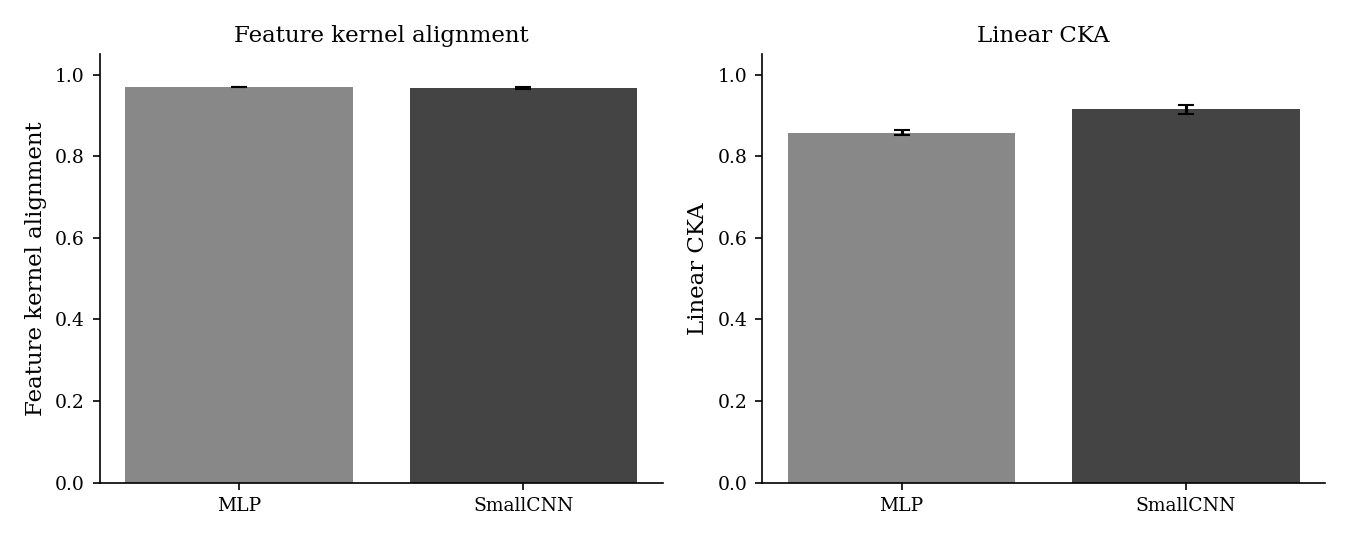
\includegraphics[width=0.55\linewidth]{figures_extended/representation_cka_bars.png}
\caption{Penultimate-layer feature similarity between matched SGD and Adam runs.}
\label{fig:representation-bars}
\end{figure}

\FloatBarrier

% =============================================================================

\section{Three-Level Synthesis}
\label{sec:three-level}

The Parts~II--IX sequence organizes evidence at three levels of geometry. Table~\ref{tab:three-level} summarizes the picture.

\begin{table}[H]
\centering
\small
\setlength{\tabcolsep}{3pt}
\begin{tabular}{p{2.4cm}p{4.8cm}p{4.5cm}p{3.5cm}}
\toprule
\textbf{Level} & \textbf{Quantities} & \textbf{What it answers} & \textbf{Verdict (this study)} \\
\midrule
Parameter geometry & $\|\theta_T-\theta_0\|_2$, $\mathcal{P}_T$, $R_T$, $\lambda_{\max}(H)$, $\operatorname{tr}(H)$, $\bar d_{\mathrm{seed}}$, $\Delta\widehat L(\sigma)$ & Where does the optimizer go, and what is the local curvature? & Adam path length $\sim 3\times$ SGD's in both architectures; directness ratio essentially equal. MLP: Adam $\sim 5$--$6\times$ flatter at matched loss. SmallCNN: ordering reverses---Adam $\sim 10\times$ \emph{sharper} at matched loss. \\
\addlinespace
Basin geometry & Linear-interpolation loss curve, barrier $B$ & Are the two solutions in the same low-loss region? & Small but reproducibly positive train barrier ($0.072$ MLP, $0.062$ CNN); test barrier $\le 0.02$. Distinct training-loss basins, near-identical population-loss landscape. \\
\addlinespace
Function and representation geometry & $D_{\mathrm{pred}}$, $D_{\mathrm{SKL}}$, $C_{\mathrm{logit}}$, $A(K_S,K_A)$, CKA & Do parameter differences correspond to different predictors or representations? & Decisions: $\sim 7\%$ disagreement and $C_{\mathrm{logit}}\approx 0.6$ in both. Representations: CKA $0.86$ MLP, $0.91$ CNN---high but not identical. Optimizer-induced functional spread is concentrated in the classifier head, not the feature space. \\
\bottomrule
\end{tabular}
\caption{Three-level synthesis of the implicit-bias evidence.}
\label{tab:three-level}
\end{table}

The data support a sharper version of the message we anticipated:
\begin{quote}
\emph{Adam substantially changes parameter-space trajectory and local Euclidean geometry, the change survives loss-matching control, and it crosses a (small) basin boundary on the training surface. But the change \textbf{compresses} as it propagates: by the function level, agreement is much closer ($\sim 93\%$); by the population-loss landscape, the two basins are essentially the same. The MLP/SmallCNN comparison shows that architecture also mediates which curvature regime each optimizer selects, with the convolutional inductive bias even reversing the flatness ordering at matched loss.}
\end{quote}

This is the core message of the extended report. Optimizer-induced parameter geometry is real and not merely a final-loss artifact; but generalization is determined by what survives at the function and representation levels, and by that point most of the parameter-space gap has been absorbed.

\FloatBarrier
\begin{figure}[H]
\centering
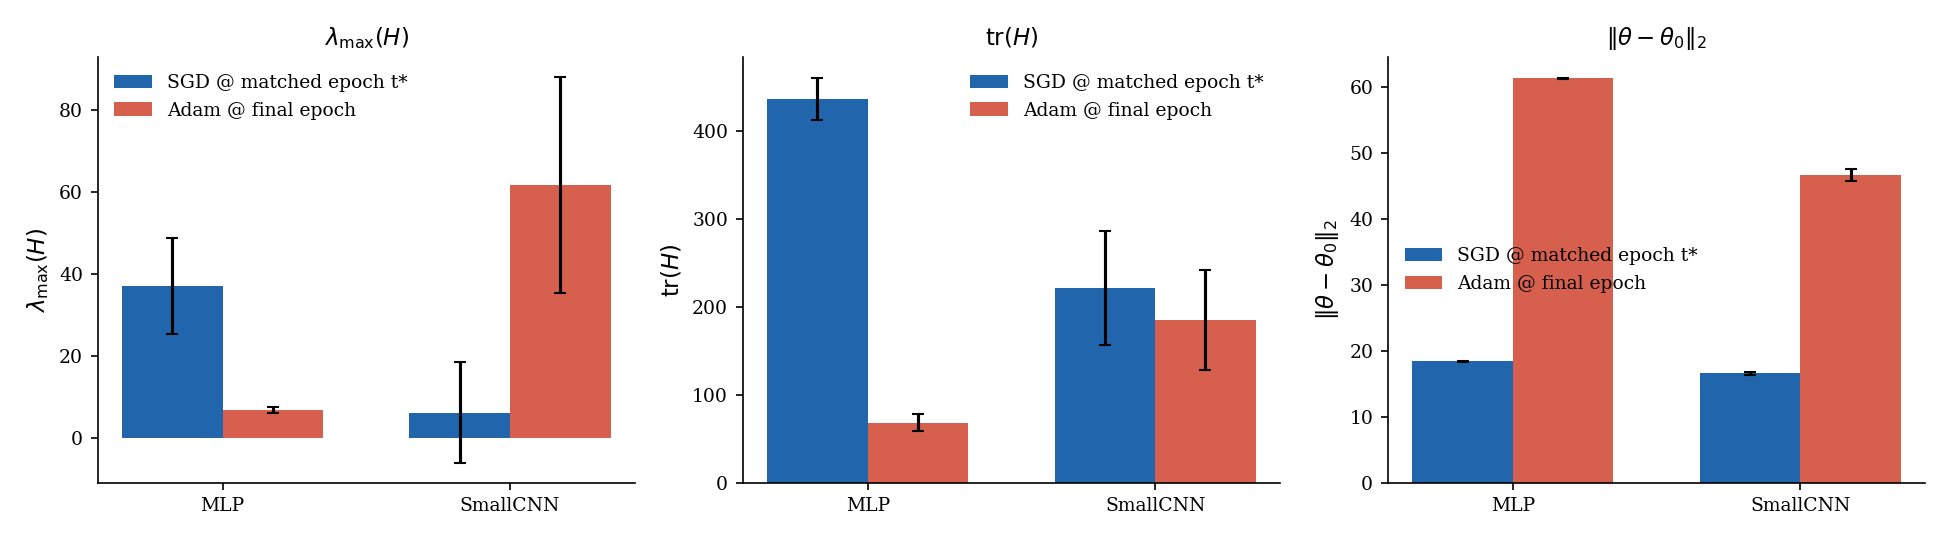
\includegraphics[width=0.85\linewidth]{figures_extended/loss_matched_summary.png}
\caption{Loss-matched geometry comparison across both architectures, summarizing $\|\theta-\theta_0\|_2$, $\lambda_{\max}(H)$, $\operatorname{tr}(H)$ and function-space disagreement.}
\label{fig:loss-matched-summary}
\end{figure}

\FloatBarrier
